\section{String Edit Distance}
{\tiny typically formulated as the (inverse) cost of obtaining one of the strings from the other through a number of edit operations \\
once we obtain the optimal edit operations, we may also be able to determine the optimal alignment between the strings}\\
\scriptsize{Hamming distance}\\ 
{\tiny number of different symbols in the corresponding positions\\
easy calculation, but cannot handle sequences of different lengths}\\
\scriptsize{Longest common subsequence (LCS)}\\
{\tiny an order-preserving sequence of symbols from a string (solved by UNIX diff)\\
e.g. LCS(hygiene, hygeine) = hygine / hygene\\
naive solution:\\
1. Enumerate all subsequences of the first string (exponential)\\
2. Check if it is also a subsequence of the second string\\
O(m2**n) for strings of size n and m\\
recursive definition:\\
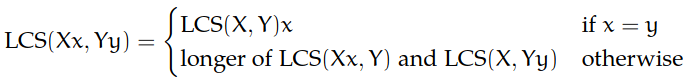
\includegraphics[scale=0.2]{lcs-recursive.png}\\
divide and conquer:\\
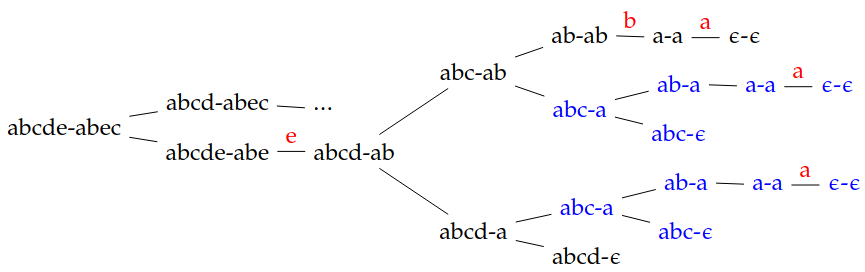
\includegraphics[scale=0.2]{lcs-divide.png}\\
dynamic programming: \\
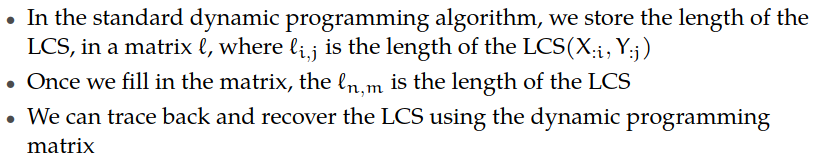
\includegraphics[scale=0.2]{lcs-dynamic.png}\\
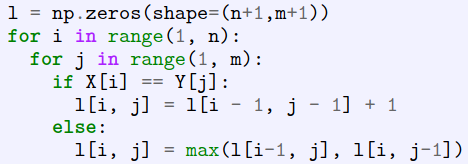
\includegraphics[scale=0.25]{lcs-algo.png}\\
time complexity O(nm), space complexity O(nm)\\
back errors give a set of edit operations (assume original string is the vertical one):\\
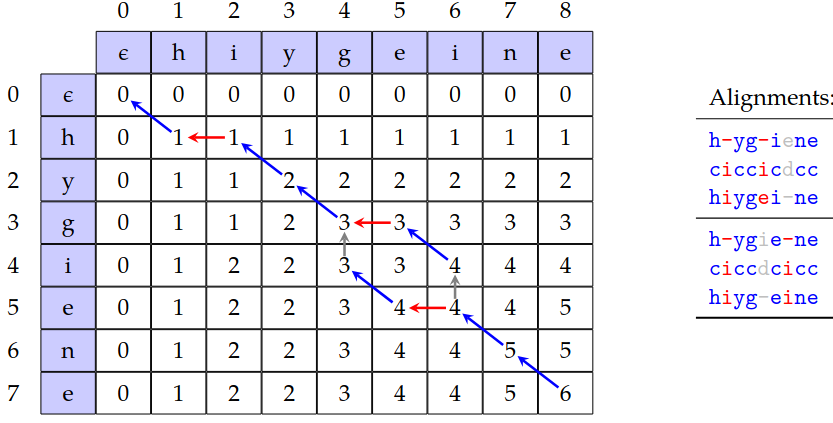
\includegraphics[scale=0.15]{lcs-recover.png}\\
- copy (diagonal arrows in the demonstration)\\
- insert (left arrows in the demo)\\
- delete (up arrows in the demo)\\
cost: copy 0, delete 1, insert 1
}\\
\scriptsize{Levenshtein distance}\\
{\tiny the total cost of insertions, deletions and substitutions\\
naive recursion as in lcs with cost 1 for all operations\\
\texttt{d[i,j]= min(d[i-1,j]+1, d[i,j-1]+1, d[i-1,j-1])}\\
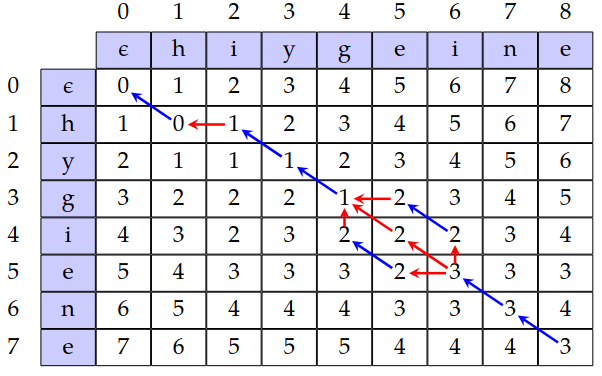
\includegraphics[scale=0.2]{levenshtein.png}
}\\
\scriptsize{swap}\\ {\tiny useful for applications like spell checking
}